\documentclass{article}
\usepackage[utf8]{inputenc}
\usepackage{geometry}
\usepackage{graphicx}
\usepackage{pgfplots}
\usepackage{verbatim}
\usepackage{amssymb}
\usepackage{amsmath}
\usepackage{tcolorbox} %needed
\usepackage{comment}
\tcbuselibrary{listingsutf8}
\usepackage{hyperref}

\geometry{a4paper, left=2cm, right=2cm, top=1cm, bottom=2cm}
\pgfplotsset{compat=1.18}

\begin{document}

\section*{Demostración gráfica de cada uno de los incisos}\\
\textit{Nota: El enlace de Desmos requiere clickear el símbolo de "play" para oscilar valores entre los ejes mayores y menores, en el apartado de funciones se detalla esta gráfica.}\\\\
Ejercicio I. \href{https://www.geogebra.org/m/txb4xqs5}{https://www.geogebra.org/m/txb4xqs5} \\
Ejercicio II. \href{https://www.geogebra.org/m/gx9gxwxk}{https://www.geogebra.org/m/gx9gxwxk} \\
Ejercicio III \href{https://www.geogebra.org/m/gwjagzbw}{https://www.geogebra.org/m/gwjagzbw}\\
Ejercicio V \href{https://www.desmos.com/calculator/vhcwo1h5li?lang=es}{https://www.desmos.com/c/vhcwo1h5li} \\
Ejercicio VI \href{https://www.geogebra.org/m/x37hyj4q}{https://www.geogebra.org/m/x37hyj4q} \\
Ejercicio VII \href{https://www.geogebra.org/m/b84hbbzt}{https://www.geogebra.org/m/b84hbbzt} \\
Ejercicio X \href{https://www.geogebra.org/m/juwn4qhs}{https://www.geogebra.org/m/juwn4qhs} \\
Ejercicio XI \href{https://www.geogebra.org/m/r8kq3gsm}{https://www.geogebra.org/m/r8kq3gsm} \\
Ejercicio XII \href{https://www.geogebra.org/m/n2srgyrw}{https://www.geogebra.org/m/n2srgyrw} \\

\begin{figure} [h]
    \centering
    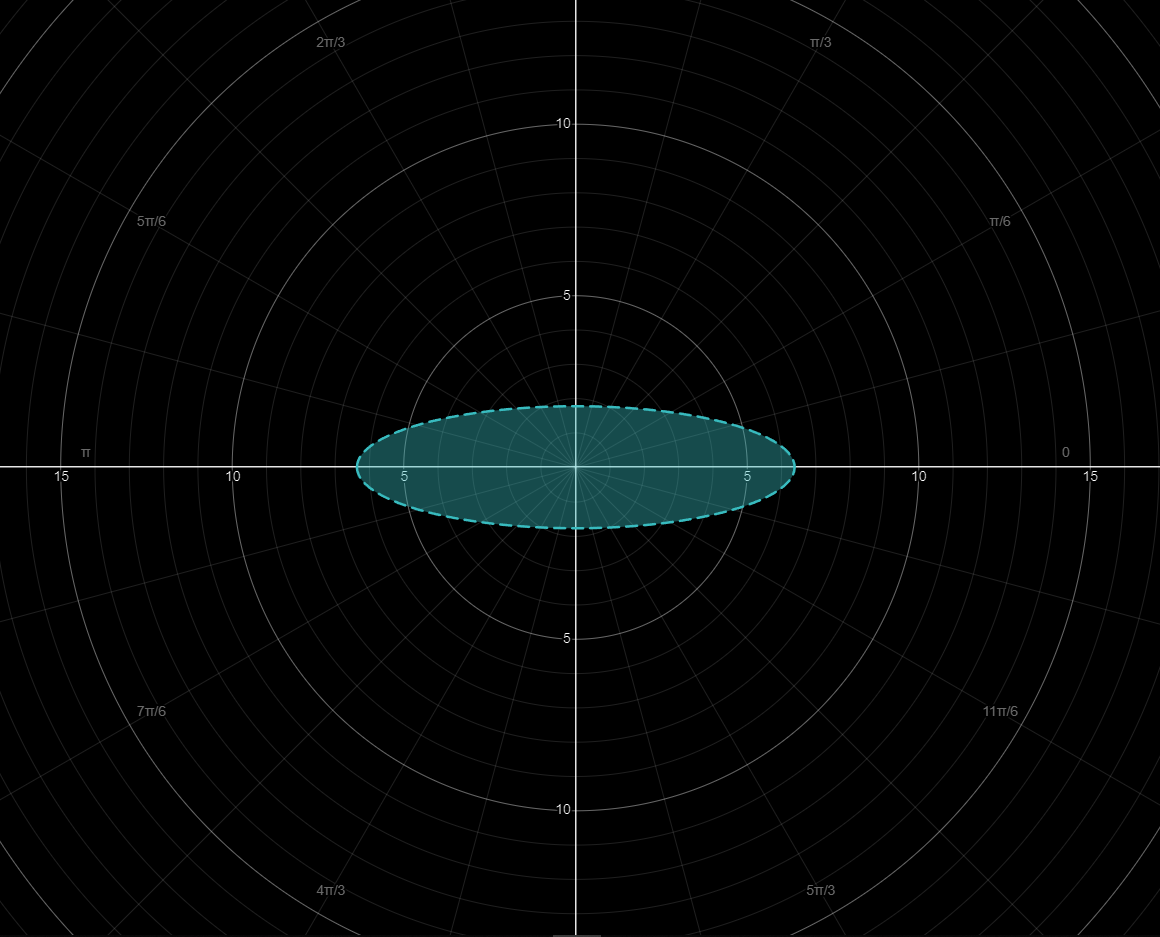
\includegraphics[width=1\linewidth]{Desmos.png}
    \caption{Elipse de ejes cambiantes en modo oscuro de Desmos.}
    \label{fig:enter-label}
\end{figure}


\end{document}